\section{Client GUI}
\label{guiimpl}

As we implemented the GUI, the actual GUI layout changed from our original wireframes in various ways. Java Swing introduced some problems with parts of our design and we had to change it to accommodate. We also chose to add more features over time.

In the main window, there have been a few deviations from the original wireframes (see figure \ref{MainWindowDia}). We chose to show each user's display picture and personal message by their name, to increase the usefulness of the contact list. We then pushed the status icons to the right side of the window to avoid crowding. We also changed the layout for offline/online users. They were going to be expandable, like a JTree would be layed out, but because of the issues described in section \ref{code_evol} we were forced to use JLists. Viewing offline users is optional, and can be changed in the Options drop-down menu. To indicate how many users are offline or online, we now have a line at the top of the contact list that updates as friends go online/offline.

\begin{figure}
    \begin{center}
        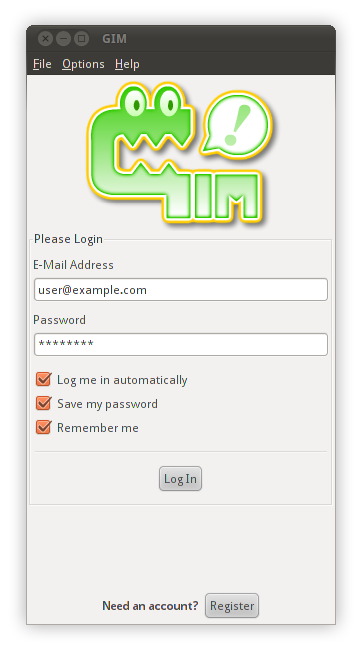
\includegraphics[scale=0.6]{Implementation/diagrams/login.png}
        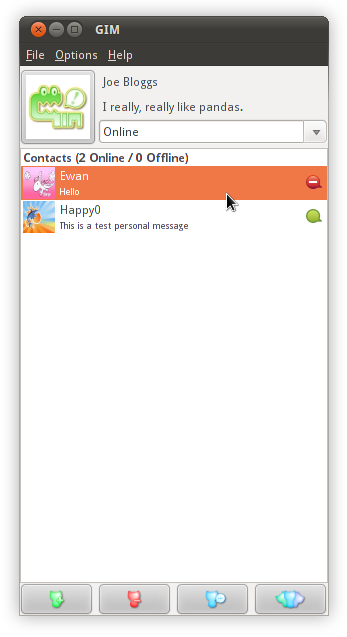
\includegraphics[scale=0.6]{Implementation/diagrams/main.png}
        \caption{The login panel and main window of the GIM Client.}
        \label{MainWindowDia}
    \end{center}
\end{figure}

There were also changes to the chat window (see figure \ref{ChatWindowDia}). We added the status of the contact beside their name at the top of the window. The buttons below the chat box for emoticons/smileys, file transfers, and group chat are all gone. Emoticons are instead automatic, in that when a series of characters such as `:)' is sent as a message, the picture of a cartoon smiling face, for example, is put in place of those characters. As for the other buttons, we did not have time to implement file transfers, and we decided that the group chat button on the main window was enough.

\begin{figure}
    \begin{center}
        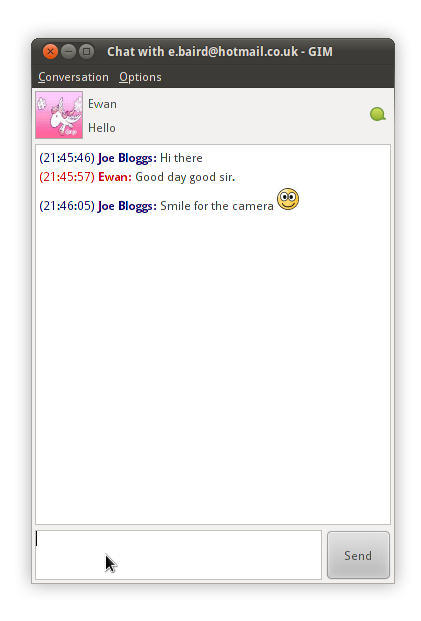
\includegraphics[scale=0.5]{Implementation/diagrams/single_chat.png}
        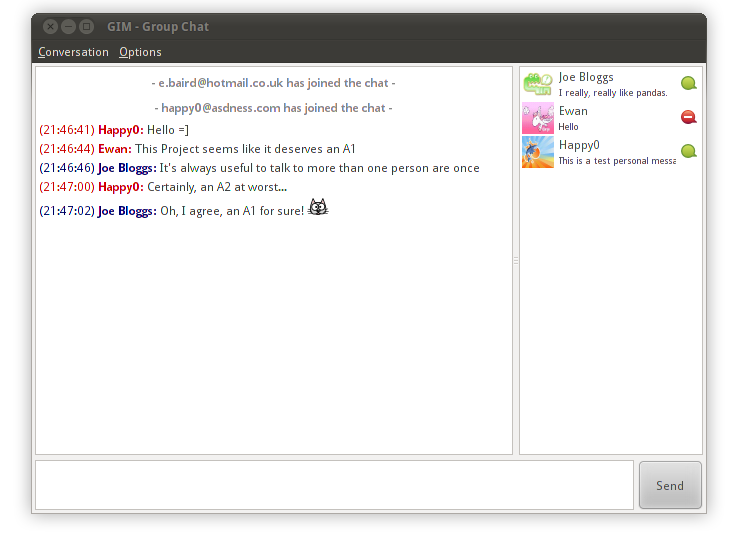
\includegraphics[scale=0.5]{Implementation/diagrams/group_chat.png}
        \caption{Examples of single and group chat windows in GIM.}
        \label{ChatWindowDia}
    \end{center}
\end{figure}

The menus at the top of the windows ended up being changed. The main window's menus stayed the same (File, Options, and Help), except that when you click on the Options menu, a list of checkboxes appears instead of the more complex panel we had planned. For a while we had the exact same menus for both the main window and chat windows, but then we decided it would be confusing to have more than one place to change the same options (more details about how menus have changed are in section \ref{designimpl}). Now, the chat window has a Conversation menu and an Options menu. The Options menus in the chat window and main window are different, offering options that correspond to the window it's in. To explain, the main window's changeable options are ``Show Offline Users'' and ``Show Notifications,'' while the chat window's options are ``Enable Logging'' and ``Show Timestamps.'' The Conversation menu has items like ``View Log,'' ``Clear Window,'' and ``Block.''

